%%%%%%%%%%%%%%%%%%%%%%%%
% 06. Februar 2024
%%%%%%%%%%%%%%%%%%%%%%%%

\thispagestyle{pagenumberonly}

\subsection{Ableitung als Grenzwert}

\begin{definition} % Definition 1
    \marginnote{[06. Feb]}
    Es seien $D = \pair{a,b}\sbset\R$, $x\in D$ und $f: D\fromto \R$. $f$ heißt im Punkt $x$ von rechts differenzierbar, falls
    \begin{align*}
        f'_+ &\definedas \lim_{h\fromto 0_+} \frac{f(x+h)-f(x)}{h}
        \intertext{existiert. $f$ ist von links differenzierbar, falls}
        f'_- &\definedas \lim_{h\fromto 0_-} \frac{f(x+h)-f(x)}{h}
    \end{align*}
    existiert. $f$ ist im Punkt $x$ differenzierbar, falls $f'_+$ und $f'_-$ existieren und $f'_+ = f'_-$. Das ist äquivalent zu der Existenz von
    \begin{align*}
        \lim_{\substack{h\fromto 0\\ h\neq 0}} \frac{f(x+h)-f(x)}{h}
    \end{align*}
\end{definition}

\begin{satz} % Satz 2
    \label{satz:18-2}
    Sei $a\in\pair{c,d}\sbset\R$. Die Funktion $f: \pair{c,d}\fromto\R$ ist genau dann im Punkt $a$ differenzierbar, wenn $\ex C\in\R$ mit $f(x) = f(a)+C\cdot\pair{x-a} + \varphi\of{x}$ wobei
    \begin{align*}
        \lim_{x\fromto a} \frac{\varphi\of{x}}{x-a} = 0
    \end{align*}
    \begin{proof}
        \anf{$\impl$}: Sei $f$ differenzierbar. Wir wählen $\varphi\of{x} \definedas f(x)-f(a) - f'(a)\cdot\pair{x-a}$ und $C=f'\of{a}$.
        \begin{align*}
            \lim_{x\fromto a} \frac{\varphi\of{x}}{x-a} &= \lim_{x\fromto a} \underbrace{\frac{f(x)-f(a)}{x-a}}_{\fromto f'(a)} - f'(a) = 0
        \end{align*}
        \anf{$\Leftarrow$}: Es gilt $f(x) = f(a)+C\cdot\pair{x-a} + \varphi\of{x}$ und $\frac{\varphi(x)}{x-a}\fromto 0$ für $x\fromto a$
        \begin{align*}
            &\impl \frac{f(x)-f(a)}{x-a} = C + \frac{\varphi(x)}{x-a}\\
            &\impl \abs{\frac{f(x)-f(a)}{x-a} - C} \fromto 0\\
            &\impl \frac{f(x)-f(a)}{x-a}\fromto C\\
            &\impl f \text{ ist in $a$ differenzierbar}\qedhere
        \end{align*}
    \end{proof}
\end{satz}

\begin{korollar}
    \theoremescape
    \label{korollar:abschaetzungen-ableitung}
    \begin{enumerate}[label=(\roman*)]
        \item Wenn $f$ im Punkt $a$ differenzierbar ist, dann ist $f$ im Punkt $a$ auch stetig.
        \item Sei $f'(a) \neq 0$. Dann gilt
        \begin{align*}
            \exists h_0~\forall h=x-a \text{ mit } \abs{h} < h_0,~h\neq 0\colon \abs{f(x)-f(a)}\geq\frac{1}{2}\abs{f'(a)}\cdot\abs{x-a}
        \end{align*}
        \newpage
        \item $\exists h_0$, so dass für alle $x$ mit $\abs{x-a} < h_0,~x\neq a$ gilt
        \begin{enumerate}[label=(\arabic*)]
            \item \fixedspace{6cm}{$\abs{f(x)-f(a)} \leq 2\abs{f'(a)}\cdot\abs{x-a}$} für $f'(a)\neq 0$
            \item \fixedspace{6cm}{$\abs{f(x)-f(a)} \leq \varepsilon\cdot\abs{x-a}$} für $f'(a) = 0$ \quad ($\forall\varepsilon > 0$, $h_0$ ist von $\varepsilon$ abhängig)
        \end{enumerate}
    \end{enumerate}

    \begin{proof}[Beweis (i)]
        Für $x\fromto a$ gilt
        \begin{align*}
            f(x)-f(a) &= C\cdot\underbrace{\pair{x-a}}_{\fromto 0} + \underbrace{\frac{\varphi(x)}{x-a}}_{\fromto 0}\cdot\underbrace{\pair{x-a}}_{\fromto 0}\fromto 0\qedhere
        \end{align*}
    \end{proof}

    \begin{proof}[Beweis (ii)]
        Für $x\fromto a$ gilt
        \begin{align*}
            f(x) &= f(a) + f'(a)\cdot\pair{x-a} + \frac{\varphi(x)}{x-a}\cdot\pair{x-a}\\
            \abs{f(x)-f(a)} &\geq \abs{f'(a)}\cdot\abs{x-a} - \underbrace{\abs{\frac{\varphi(x)}{x-a}}}_{\fromto 0}\cdot\abs{x-a}\geq \frac{1}{2}\cdot\abs{f'(a)}\cdot\abs{x-a}\qedhere
        \end{align*}
    \end{proof}
    \begin{proof}[Beweis (iii)]
    (1)
        Für $x\fromto a$ gilt
        \begin{align*}
            \abs{f(x)-f(a)} &\leq \abs{f'(a)}\cdot\abs{x-a} + \underbrace{\abs{\frac{\varphi(x)}{x-a}}}_{\fromto 0} \cdot \abs{x-a} \leq 2\abs{f'(a)}\cdot\abs{x-a}
            \intertext{(2)}
            \abs{f(x)-f(a)} &= \abs{\underbrace{f'(a)}_{\fromto 0} \cdot \pair{x-a} + \underbrace{\frac{\varphi(x)}{x-a}}_{\fromto 0}\cdot\pair{x-a}} \leq \varepsilon\cdot\abs{x-a}\qedhere
        \end{align*}
    \end{proof}
\end{korollar}

\subsection{Ableitungsregeln}

\begin{satz} % Satz 3
    \label{satz:ableitungsregeln}
    Seien $f, g: (a,b)\fromto \R$ differenzierbar, $\lambda\in\R$, $x\in\pair{a,b}$. Dann gilt
    \begin{enumerate}[label=(\roman*)]
        \item $\pair{f+g}'\of{x} = f'(x)+g'(x)$
        \item $\pair{\lambda\cdot f}'\of{x} = \lambda\cdot f'(x)$
        \item $\pair{f\cdot g}'\of{x} = f'(x)\cdot g(x) + g'(x)\cdot f(x)$\quad\quad(Produktregel)
    \end{enumerate}
    \begin{proof}[Beweis (iii)]
        \begin{align*}
            \pair{f\cdot g}'\of{x} &= \lim_{h\fromto 0} \frac{f(x+h)g(x+h) - f(x)g(x)}{h}\\
            &= \lim_{h\fromto 0} \frac{f(x+h)g(x+h) - f(x+h)g(x) + f(x+h)g(x) - f(x)g(x)}{h}\\
            &= \lim_{h\fromto 0} f(x+h)\cdot \underbrace{\frac{g(x+h)-g(x)}{h}}_{\fromto g'(x)} + \lim_{h\fromto 0} g(x) \cdot \underbrace{\frac{f(x+h)-f(x)}{h}}_{\fromto f'(x)}\\
            &= f(x) \cdot g'(x) + g(x)\cdot f'(x)\qedhere
        \end{align*}
    \end{proof}
\end{satz}

\begin{uebung}
    Beweisen Sie die verbleibenden Aussagen des vorherigen Satzes.
\end{uebung}

\begin{satz}[Kettenregel] % Satz 4
    \label{satz:kettenregel}
    Seien $f: \pair{a,b}\fromto \R$ und $g: (c,d)\fromto \R$ Funktionen mit $f\interv{\pair{a,b}} \sbset \pair{c,d}$. Die Funktion $f$ sei im Punkt $x\in\pair{a,b}$ differenzierbar und $g$ sei im Punkt $y\definedas f(x)$ differenzierbar. Dann gilt
    \begin{align*}
        \pair{g\circ f}'(x) = g'(f(x)) \cdot f'(x)
    \end{align*}
    \begin{proof}
        Wir definieren $F(x) \definedas g(f(x))$ und unterscheiden zwei Fälle.\\
        \textsc{Fall 1.} $f'(x) \neq 0$. Nach Korollar~\ref{korollar:abschaetzungen-ableitung} gilt
        \begin{align*}
            \ex h_0, \abs{h} < h_0\colon \abs{f(x+h)-f(x)} &\geq \frac{1}{2}\abs{f'(x)}\abs{h} \neq 0\\
            \lim_{h\fromto 0} \frac{F(x+h)-F(x)}{h} &= \lim_{h\fromto 0} \frac{\pair{F(x+h) - F(x)}\cdot\pair{f(x+h)-f(x)}}{\pair{f(x+h)-f(x)}\cdot h}\\
            &= \lim_{h\fromto 0} \frac{g(f(x+h))-g(f(x))}{f(x+h)-f(x)} \cdot \underbrace{\frac{f(x+h)-f(x)}{h}}_{\fromto f'(x)}
            \intertext{$f(x)=y$ und $f(x+h) = y + \Delta y$}
            \lim_{h\fromto 0} \frac{g(f(x+h))-g(f(x))}{f(x+h)-f(x)} &= \lim_{h\fromto 0} \frac{g(y+\Delta y) - g(y)}{\Delta y}\tag{$\Delta y \neq 0$}\\
            &= \lim_{\Delta y \fromto 0} \frac{g(y+\Delta y) - g(y)}{\Delta y}\\
            &= g'(y) = g'(f(x))\\
            \impl \frac{F(x+h)-F(x)}{h} &\fromto g'(f(x)) \cdot f'(x)
            \intertext{\textsc{Fall 2.} $f'(x) = 0$. Dann gilt nach Korollar~\ref{korollar:abschaetzungen-ableitung}}
            \abs{\frac{g(f(x+h)) - g(f(x))}{h}} &\leq \frac{c\cdot\abs{f(x+h)-f(x)}}{h}\\
            &\leq \frac{c\cdot\varepsilon\cdot \abs{x+h-x}}{h}\\
            &= c\cdot\varepsilon\\
            \intertext{mit $c=\max\set{2\cdot\abs{g'(f(x))}, 1}$ und $\varepsilon$ beliebig klein}
            \impl \lim_{h\fromto 0} \frac{F(x+h)-F(x)}{h} = 0 &= g'\of{f\of{x}} \cdot 0 = g'\of{f\of{x}}\cdot f'\of{x}\\
            \intertext{Damit folgt insgesamt}
            \pair{g\circ f}'(x) &= g'(f(x))\cdot f'(x)\qedhere
        \end{align*}
    \end{proof}
\end{satz}

\begin{satz}[Quotientenregel] % Satz 5
    \label{satz:quotient-ableitung}
    Für zwei differenzierbare Funktionen $u,v$ gilt
    \begin{align*}
        \pair{\frac{v}{u}}' = \frac{v'\cdot u - u'\cdot v}{u^2}
    \end{align*}
    \begin{proof}
        \begin{align*}
            \pair{\frac{v}{u}}' &= \pair{v\cdot\frac{1}{u}}' = v'\cdot \frac{1}{u} + v\cdot\frac{1}{u^2}\cdot u'\cdot (-1) = \frac{v'u - u'v}{u^2}\qedhere
        \end{align*}
    \end{proof}
\end{satz}

\begin{beispiel}[Ableitung der Exponentialfunktion]
    Es sei $a\in\C$, $x\in\R$. Wir wollen $e^{ax}$ ableiten
    \begin{align*}
        \pair{e^{ax}}' &= \lim_{h\fromto 0} \frac{e^{a(x+h)} - e^{ax}}{h} = \lim_{h\fromto 0}e^{ax} \cdot \frac{e^{ah}-1}{h} = e^{ax}\cdot \lim_{h\fromto 0} \frac{e^{ah}-1}{h}\\
        e^{ah} &= \sum_{n=0}^{\infty} \frac{(ah)^n}{n!} = 1 + ah + (ah)^2\cdot\sum_{n=2}^{\infty} \frac{(ah)^{n-2}}{n!}
        \intertext{Wir schätzen den letzten Teil der Gleichung mit $\abs{h} < \frac{1}{\abs{a}}$ ab}
        \abs{ \sum_{n=2}^{\infty} \frac{(ah)^{n-2}}{n!}} &\leq \sum_{n=2}^{\infty} \frac{1}{n!} < e\\
        \impl \pair{e^{ax}}' &= e^{ax}\cdot \lim_{h\fromto 0} \frac{1+ah+(ah)^2\cdot e - 1}{h} = a\cdot e^{ax}\tag{$a\in\C$}
    \end{align*}
\end{beispiel}

%%%%%%%%%%%%%%%%%%%%%%%%
% 08. Februar 2024
%%%%%%%%%%%%%%%%%%%%%%%%

\begin{beispiel}[Ableitung von $\sin$ und $\cos$]
    \marginnote{[08. Feb]}
    \begin{align*}
        \pair{\sin x}' &= \pair{\Im e^{ix}}' = \Im \pair{e^{ix}}' = \Im\pair{i\cdot e^{ix}} = \Im\of{i\cdot\pair{\cos x + i\cdot \sin x}} = \cos x
        \intertext{Analog lässt sich zeigen, dass gilt}
        \pair{\cos x}' &= -\sin x
    \end{align*}
\end{beispiel}
\begin{beispiel}[Ableitung von $\tan$]
    \begin{align*}
        \pair{\tan x}' &= \pair{\frac{\sin x}{\cos x}}' = \frac{\cos x \cdot \cos x -\pair{-\sin x \cdot \sin x}}{\cos^2 x} = \frac{\cos^2 x + \sin^2 x}{\cos^2 x} = \frac{1}{\cos^2 x}
    \end{align*}
\end{beispiel}

\begin{satz}[Ableitung der Umkehrfunktion] % Satz 6
    \label{satz:ableitung-umkehrfunktion}
    Sei $f: \pair{a,b} \fromto \pair{c,d}$ eine bijektive Abbildung, die im Punkt $x\in\pair{a,b}$ differenzierbar ist. Dann ist die Funktion $f^{-1}$ an der Stelle $y=f\of{x}$ differenzierbar und es gilt
    \begin{align*}
        \pair{f^{-1}}'\of{y} = \frac{1}{f'\of{x}}
    \end{align*}
    \begin{proof}
        \begin{align*}
            \pair{f^{-1}}'\of{y} &= \lim_{h\fromto 0} \frac{\overbrace{f^{-1}\of{y+h}}^{\definedasbackwards \xi} - f^{-1}\of{y}}{h} = \lim_{h\fromto 0}\frac{\xi - x}{f\of{\xi} - f\of{x}}\\
            &= \lim_{h\fromto 0} \frac{1}{\frac{f\of{\xi} - f\of{x}}{\xi-x}} = \frac{1}{\lim_{h\fromto 0} \frac{f\of{\xi} - f\of{x}}{\xi-x}}
            \intertext{Wegen der Monotonie und Stetigkeit von $f$ können wir umformen zu}
            &= \frac{1}{\lim_{\xi\fromto x} \frac{f\of{\xi} - f\of{x}}{\xi-x}} = \frac{1}{f'\of{x}}\qedhere
        \end{align*}
    \end{proof}
\end{satz}

\begin{beispiel}[Ableitung des Logarithmus]
    Wir definieren $f\definedas e^x$. Damit gilt
    \begin{align*}
        \log y &= f^{-1}\of{y}\\
        \log\pair{e^x} &= x\\
        \pair{\log y}' &= \frac{1}{\pair{e^x}'_{\lvert y=e^x}} = \frac{1}{\pair{e^x}_{\lvert y=e^x}} = \frac{1}{y}
    \end{align*}
\end{beispiel}

\begin{bemerkung}[Ableitung von Potenzen]
    \footnote{In VL erst im nächsten Unterkapitel behandelt}
    \begin{align*}
        \pair{x^{\alpha}}' &= \pair{e^{\log x^{\alpha}}} = \pair{e^{\alpha\log x}}'
        \intertext{Nach Satz~\ref{satz:kettenregel}}
        &= e^{\alpha \log x} \cdot \alpha \cdot \pair{\log x}' = \frac{\alpha x^{\alpha}}{x} = \alpha \cdot x^{\alpha-1}
    \end{align*}
\end{bemerkung}

\begin{beispiel}[Ableitung von $\arccos$]
    Es sei $y\in\pair{-1, 1}$. Dann gilt
    \begin{align*}
        \pair{\arccos y}' &= \frac{1}{\pair{\cos x}'_{\lvert \cos x = y}} = \frac{1}{-\sin\of{\arccos\of{y}}}\\
        &= \frac{1}{\pm\sqrt{1-\cos^2\of{\arccos y}}} = \pm \frac{1}{\sqrt{1-y^2}}
    \end{align*}
\end{beispiel}

\subsection{Lokale Extrema und Mittelwertsätze}

\begin{definition}[Lokales Maximum und Minimum] % Definition 7
    Sei $f: \pair{a,b} \fromto\R$. Man sagt $f$ habe in $x\in\pair{a,b}$ ein lokales Maximum (Minimum), wenn ein $\varepsilon > 0$ existiert, so dass
    \begin{align*}
        f\of{x} \underset{(\leq)}{\geq} f\of{\xi}\quad \forall \xi\in\pair{x-\varepsilon, x+\varepsilon}
    \end{align*}
\end{definition}

\begin{satz}[Ableitung bei lokalen Extrema]
    \label{satz:ableitung-extrem}
    Sei $f: \pair{a,b} \fromto \R$ differenzierbar und $x\in\pair{a,b}$ ein lokales Extremum. Dann gilt $f'\of{x} = 0$.
    \begin{proof}
        $\ex \varepsilon > 0$, $f\of{\xi} \leq f\of{x}$, $\xi\in\pair{x-\varepsilon, x+\varepsilon}$
        \begin{align*}
            f'_{+}\of{x} &= \lim_{\substack{\xi\fromto x\\ \xi > x}} \frac{f\of{\xi} - f\of{x}}{\xi - x} \leq 0\\
            f'_{-}\of{x} &= \lim_{\substack{\xi\fromto x\\ \xi < x}} \frac{f\of{\xi} - f\of{x}}{\xi - x} \geq 0\\
            \impl f'_{+} &= f'_{-} = 0\qedhere
        \end{align*}
    \end{proof}
\end{satz}

\begin{bemerkung}
    Die Umkehrung gilt nicht. Wir betrachten $f: x\mapsto x^3$ mit $f'(0) = 3x^2 = 0$, aber die Funktion hat an der Stelle $x=0$ kein lokales Maximum oder Minimum.
\end{bemerkung}

\begin{bemerkung}
    Sei $f$ auf $\interv{a,b}$ stetig und auf $\pair{a,b}$ differenzierbar. Dann kann das Maximum/Minimum der Funktion auch auf den Intervall-Grenzen $a$ und $b$ liegen, obwohl die Ableitung für diese nicht bestimmbar ist.
\end{bemerkung}

\begin{satz}[Satz von Rolle]
    \label{satz:von-rolle}
    Sei $a < b$, $f: \interv{a,b} \fromto \R$ eine stetige Funktion mit $f(a) = f(b)$. Die Funktion $f$ sei in $\pair{a,b}$ differenzierbar. Dann $\ex\xi\in\pair{a,b}$ mit $f'\of{\xi} = 0$.
    \begin{proof}
        ~\\
        \textsc{Fall 1.} $f$ ist eine konstante Funktion. Dann gilt $f' = 0$.\\
        \textsc{Fall 2.} $f$ ist keine konstante Funktion. Das heißt nach Satz~\ref{satz:weierstrass-maximum-minimum} $\exists x$ mit $f\of{x} \neq f\of{a}$. Wenn $f(x) > f(a)$, dann existiert ein lokales Maximum bei $x_0\in\pair{a,b}$ und wenn $f(x) < f(a)$, dann existiert ein lokales Minimum bei $x_0\in\pair{a,b}$. Damit ist $f'\of{x_0} = 0$.
    \end{proof}
\end{satz}

\newpage

\begin{satz}[Mittelwertsatz]
    \label{satz:mittelwertsatz}
    Sei $a < b$, $f:\interv{a,b}\fromto\R$ stetig und in $\pair{a,b}$ differenzierbar. Dann gilt
    \begin{align*}
        \ex\xi\in\pair{a,b}\colon f\of{b} - f\of{a} = f'\of{\xi}\cdot\pair{b-a}
    \end{align*}
    \begin{proof}
        \begin{align*}
            F(x) &\definedas f(x) - \frac{f\of{b}-f\of{a}}{b-a}\cdot\pair{x-a}\\
            F(a) &= f(a) - \frac{f(b)-f(a)}{b-a}\cdot 0 = f(a)\\
            F(b) &= f(b) - \frac{f(b)-f(a)}{b-a}\cdot\pair{b-a} = f\of{a}\\
            \impl F(a) &= F(b)
            \intertext{Damit gilt nach Satz~\ref{satz:von-rolle}}
            \impl \ex\xi \text{ mit } F'\of{\xi} &= 0\\
            \impl f'\of{\xi} - \frac{f\of{b} - f\of{a}}{b-a} &= 0\\
            \impl f(b) - f(a) &= f'\of{\xi}\cdot\pair{b-a}\qedhere
        \end{align*}
    \end{proof}
\end{satz}

\begin{visualisierung}[Geometrische Anschauung des Mittelwertsatzes]
    Der Mittelwertsatz sagt aus, dass es einen Punkt auf jeder differenzierbaren Funktion gibt, dessen Tangente parallel zu einer affin-linearen Funktion durch $f(a)$ und $f(b)$ läuft.
    \begin{figure}[H]
        \centering
        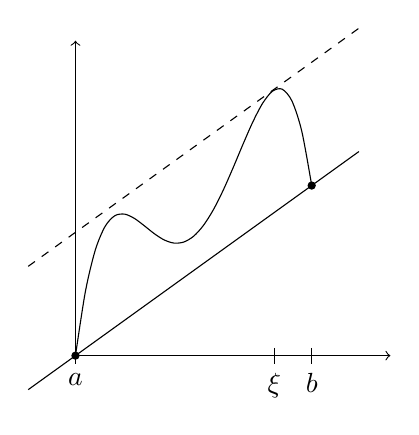
\begin{tikzpicture}
            \draw[->] (0, 0) -- (4, 0);
            \draw[->] (0, 0) -- (0, 4);
            \draw (0, 0.1) -- (0, -0.1) node[below] {$a$};
            \draw (4.21*.6, 0.1) -- (4.21*.6, -0.1) node[below] {$\xi$};
            \draw (5*.6, 0.1) -- (5*.6, -0.1) node[below] {$b$};
            \fill (0,0) circle[radius=1.5pt];
            \fill (5*.6,6*0.6*0.6) circle[radius=1.5pt];
            \draw[scale=0.6, domain=0:5, smooth, variable=\x] plot ({\x}, {(-43/120 *\x*\x*\x*\x+71/20*\x*\x*\x-1337/120*\x*\x+259/20*\x)*0.6});
            \draw[scale=0.6, domain=-1:6, smooth, variable=\x] plot ({\x}, {(\x*6/5)*0.6});
            \draw[scale=0.6, domain=-1:6, smooth, variable=\x, dashed] plot ({\x}, {(\x*6/5+4.35)*0.6});
        \end{tikzpicture}
        \caption{Tangente an der Stelle $x=\xi$\\parallel zur Geraden durch die beiden Punkte}
    \end{figure}
\end{visualisierung}

\begin{korollar} % Korollar 10
    Es gilt genau dann $f'(x) = 0$ für alle $x\in\pair{a,b}$, wenn $f(x)$ eine konstante Funktion in $\interv{a,b}$ ist.
    \begin{proof}
        \begin{align*}
            f(x_1) - f(x_2) \annot[{&}]{=}{\ref{satz:mittelwertsatz}} f'\of{\xi}\cdot\pair{x_1 - x_2}\\
            &= 0\cdot\pair{x_1 - x_2}\\
            \impl f(x_1) &= f(x_2)\qedhere
        \end{align*}
    \end{proof}
\end{korollar}

\begin{satz} % Satz 11
    \label{satz:18-11}
    Seien $f$ und $g$ stetig auf $\interv{a,b}$ und auf $\pair{a,b}$ differenzierbar. Dann gilt
    \begin{align*}
        \ex\xi\in\pair{a,b}\colon \interv{f(b)-f(a)}\cdot g'\of{\xi} &= \interv{g(b)-g(a)}\cdot f'\of{\xi}
    \end{align*}
    \begin{proof}
        \begin{align*}
            h(t) &\definedas \interv{f(b)-f(a)}\cdot g(t) - \interv{g(b)-g(a)}\cdot f(t)\\
            \impl h(a) &= h(b)\\
            \annot{\impl}{\ref{satz:mittelwertsatz}} \ex \xi \in\pair{a,b} &\text{ mit } h'\of{\xi} = 0\\
            \impl \interv{f(b)-f(a)}\cdot g'\of{\xi} &- \interv{g(b)-g(a)}\cdot f'\of{\xi} = 0\\
            \impl \interv{f(b)-f(a)}\cdot g'\of{\xi} &= \interv{g(b)-g(a)}\cdot f'\of{\xi}\qedhere
        \end{align*}
    \end{proof}
\end{satz}

\begin{notation}[Ableitungen höherer Ordnung] % Definition 11
    Wir definieren für die zweite Ableitung
    \begin{align*}
        f'' &= \pair{f'}'
        \intertext{und allgemein}
        f^{(n)} &= \pair{f^{(n-1)}}'
    \end{align*}
\end{notation}

\begin{satz}[Der Taylorsche Satz] % Satz 12
    \label{satz:taylor}
    Es sei $f$ eine reelle Funktion auf $\interv{a,b}$ und $f^{(n-1)}$ sei stetig auf $\interv{a,b}$ und $f^{(n)}$ existiere auf $\pair{a,b}$. Sei $\pair{\alpha,\beta}\subseteq \interv{a,b}$ und
    \begin{align*}
        P_{n-1}(t) &= \sum_{k=0}^{n-1} \frac{f^{(k)}\of{\alpha}}{k!}\cdot\pair{t-\alpha}^k\tag{\footnotemark}
        \intertext{Dann $\ex\xi\in\pair{\alpha,\beta}$ so dass}
        f\of{\beta} &= P_{n-1}\of{\beta} + \frac{f^{(n)}\of{\xi}}{n!}\cdot\pair{\beta-\alpha}^n
    \end{align*}

    \footnotetext{In manchen Lehrbüchern wird auch $T_n\of{f,\alpha}$ als alternative Schreibweise zu $P_{n}\of{t}$ verwendet.}

    %%%%%%%%%%%%%%%%%%%%%%%%
    % 13. Februar 2023
    %%%%%%%%%%%%%%%%%%%%%%%%

    \begin{proof}
        \marginnote{[13. Feb]}
        \begin{align*}
            M&\definedas \frac{f(\beta)-P_{n-1}\of{\beta}}{\pair{\beta-\alpha}^n}\tag{$M\in\R$}\\
            g(t) &\definedas f(t)-P_{n-1}\of{t} - M \cdot \pair{t-\alpha}^n\tag{$\alpha\leq t\leq\beta$}\\
            g\of{\alpha} &= f\of{\alpha} - \overbrace{0 - f\of{\alpha}}^{P_{n-1}\of{\alpha}} - 0 = 0\\
            g'\of{\alpha} &= f'\of{\alpha} - f'\of{\alpha} = 0\\
            \vdots&\\
            g^{(n-1)}\of{\alpha} &= 0\\[10pt]
            g\of{\beta} &= f\of{\beta} - P_{n-1}\of{\beta} - \frac{f\of{\beta} - P_{n-1}\of{\beta}}{\pair{\beta-\alpha}^n}\cdot \pair{\beta-\alpha}^n = 0
            \intertext{1. Schritt}
            g\of{\alpha} &= 0,~g\of{\beta} = 0
            \intertext{Nach Satz~\ref{satz:von-rolle}}
            \impl \ex x_1\in\pair{\alpha, \beta}\colon g'(x_1) &= 0
            \intertext{2. Schritt}
            g'\of{\alpha} &= 0,~g'\of{x_1} = 0\\
            \impl \ex x_2\in\pair{\alpha, x_1}\colon g''(x_2) &= 0\\[10pt]
            g''(\alpha) &= 0,~g''\of{x_2} = 0\\
            \vdots\\
            \impl\ex x_n \in\pair{\alpha, x_{n-1}}\colon g^{(n)}\of{x_n} &= 0\tag{$\xi\definedas x_n$}\\
            \impl g^{(n)}\of{\xi} = f^{(n)}\of{\xi} - 0 - M\cdot n! &= 0\\
            \equivalent M = \frac{f^{(n)}\of{\xi}}{n!} &= \frac{f\of{\beta}-P_{n-1}\of{\beta}}{\pair{\beta-\alpha}^n}\\
            \equivalent f\of{\beta} - P_{n-1}\of{\beta} &= \frac{f^{(n)}\of{\xi}}{n!}\cdot\pair{\beta-\alpha}^n\\
            f\of{\beta} &= P_{n-1}\of{\beta} + \frac{f^{(n)}\of{\beta}}{n!}\pair{\beta-\alpha}^n\qedhere
        \end{align*}
    \end{proof}
\end{satz}

\begin{bemerkung}
    Der Taylorsche Satz ist eine Verallgemeinerung des Mittelwertsatzes für höhere Ableitungen.
\end{bemerkung}

\begin{korollar}[Monotonie] % Korollar 14
    \label{korollar:monotonie}
    Sei $f$ auf $\pair{a,b}$ differenzierbar mit $f' > 0$ ($f' < 0$). Dann ist $f$ streng monoton wachsend (fallend) auf $\pair{a,b}$.
    \begin{proof}
        Seien $x_1, x_2\in\pair{a,b}$ mit $x_2 > x_1$. Nach Satz~\ref{satz:mittelwertsatz} gilt
        \begin{align*}
            f(x_2) - f(x_1) &= \underbrace{f'(\xi)}_{> 0}\cdot\underbrace{\pair{x_2 - x_1}}_{> 0} > 0\qedhere
        \end{align*}
        Der Beweis für fallende Funktionen funktioniert analog.
    \end{proof}
\end{korollar}

\begin{bemerkung}[Über Max und Min]
    Es seien $f$ differenzierbare Funktion und $x_0$ lokales Extremum von $f$ und sei $f''\of{x_0}$ existent und positiv (negativ). Dann ist $x_0$ ein lokales Minimum (Maximum).

    \begin{proof}
        \begin{align*}
            f''\of{x_0} &= \lim_{\xi\fromto x_0} \frac{f'\of{\xi} - f'\of{x_0}}{\xi-x_0} > 0\\
            &\impl \ex\varepsilon > 0\colon \frac{f'\of{\xi} - f'\of{x_0}}{\xi-x_0} > 0\quad\forall\xi, 0 < \abs{x_0-\xi} < \varepsilon\\
            &\impl \begin{cases}
                       f'\of{\xi} < 0 \text{ für } \xi < x_0~\leadsto \text{ Funktion fällt}\\
                       f'\of{\xi} > 0 \text{ für } \xi > x_0~\leadsto \text{ Funktion steigt}
            \end{cases}
        \end{align*}
        Da die Funktion vor $x_0$ fällt und danach steigt, ist $x_0$ ein lokales Minimum.
    \end{proof}
\end{bemerkung}

\newpage

\subsection{Die Regel von l'Hospital}

\begin{satz}[Regel von de l'Hospital] % Satz 16
    \label{satz:l-hospital}
    Seien $f$ und $g$ differenzierbar in $\pair{a,b}$. Sei ferner $g'\of{x} \neq 0$ für alle $x\in\pair{a,b}$ und es gelte
    \begin{align*}
        \frac{f'(x)}{g'(x)} &\fromto A \text{ für } x \fromto a\tag{1}
        \intertext{Außerdem gelte}
        f(x) \fromto 0 \text{ und } g(x)&\fromto 0 \text{ für } x\fromto a\tag{2.1}
        \intertext{\underline{oder}}
        g(x)&\fromto \infty \text{ für } x\fromto a\tag{2.2}
        \intertext{Dann gilt}
        \frac{f(x)}{g(x)}&\fromto A \text{ für } x\fromto a
    \end{align*}
    Die analoge Behauptung ist wahr für $x\fromto b$ oder für $g(x)\fromto -\infty$. Außerdem ist $g'(a) = 0$ bei der Anwendung des Satzes erlaubt.

    \begin{proof}
        Sei $A < \infty \impl\ex q> A$. Sei $A < r < q$
        \begin{align*}
            \impl \frac{f'(x)}{g'(x)} &< r \text{ für } a < x < a + \varepsilon_0
            \intertext{Nach Satz~\ref{satz:18-11} gilt mit $a < x < y < a + \varepsilon_0$}
            \frac{f(x)-f(y)}{g(x)-g(y)} &= \frac{f'(\xi)}{g'(\xi)}  < r
            \intertext{\textsc{Fall 1.} $f(x)\fromto 0$, $g(x)\fromto 0$ für $x\fromto a$}
            \impl g(y) \neq 0, \text{ weil } g(a) &= 0,~g'(a)\neq 0\\
            \lim_{x\fromto a} \frac{\overbrace{f(x)}^{\fromto 0}-f(y)}{\underbrace{g(x)}_{\fromto 0}-g(y)} &= \lim_{x\fromto a} \frac{f(y)}{g(y)} \leq r < q\\
            \impl \fa a < y < a + \varepsilon_0\colon \frac{f(y)}{g(y)} &< q\\
            \impl \lim_{y\fromto a} \frac{f(y)}{g(y)} &< q
            \intertext{\textsc{Fall 2.} $g(x)\fromto\infty$ für $x\fromto a$. Dann gilt mit $a < x < y < a + \varepsilon_0$}
            \frac{f(x)-f(y)}{g(x)-g(y)} &< r\\
            \impl \frac{\frac{f(x)}{g(x)}- \frac{f(y)}{g(x)}}{1 - \frac{g(y)}{g(x)}} &< r\\
            \impl \frac{\frac{f(x)}{g(x)}}{1} &\leq r < q\\
            \impl\fa q > A\colon \frac{f(x)}{g(x)} &< q\tag{$a<x<a+\varepsilon_0$}
        \end{align*}
        \newpage
        \noindent In beiden Fällen ist der Quotient durch $q$ nach oben beschränkt. Sei $A > -\infty$
        \begin{align*}
            \impl\exists p\colon p &< r < A\\
            \impl \frac{f(x)-f(y)}{g(x)-g(y)} &= \frac{f'\of{\xi}}{g'\of{xi}} > r > p \tag{$a < x < y < a + \varepsilon_0$}
            \intertext{Mit der gleichen Argumentation wie davor ergibt sich}
            \frac{f(x)}{g(x)} &> p \impl \frac{f(x)}{g(x)} \fromto A&&\qedhere
        \end{align*}
    \end{proof}
\end{satz}

\begin{beispiel}
    \begin{align*}
        \lim_{x\fromto 1_-} \interv{\ln x \cdot \ln\of{1-x}} &= \lim_{x\fromto 1_-} \frac{\ln\pair{1-x}}{\frac{1}{\ln\of{x}}} \annot{=}{\ref{satz:l-hospital}} \lim_{x\fromto 1_-} \frac{\frac{1}{1-x}\cdot\pair{-1}}{-\frac{1}{\ln^2\of{x}} \cdot \frac{1}{x}}\\[4pt]
        &= \lim_{x\fromto 1_-} \frac{x\cdot\ln^2\of{x}}{1-x} = \lim_{x\fromto 1_-} \frac{\ln^2\of{x}}{1-x}\\[4pt]
        \annot[{&}]{=}{\ref{satz:l-hospital}} \lim_{x\fromto 1_-} \frac{2\ln\of{x}\cdot \frac{1}{x}}{-1} = 0
    \end{align*}
\end{beispiel}

\newpage